\documentclass[a4paper]{jsarticle}
\setlength{\topmargin}{-20.4cm}
\setlength{\oddsidemargin}{-10.4mm}
\setlength{\evensidemargin}{-10.4mm}
\setlength{\textwidth}{18cm}
\setlength{\textheight}{26cm}

\usepackage[top=15truemm,bottom=25truemm,left=20truemm,right=20truemm]{geometry}
\usepackage[latin1]{inputenc}
\usepackage{amsmath}
\usepackage{amsfonts}
\usepackage{amssymb}
\usepackage[dvipdfmx]{graphicx}
\usepackage[dvipdfmx]{color}
\usepackage{listings}
\usepackage{listings,jvlisting}
\usepackage{geometry}
\usepackage{framed}
\usepackage{color}
\usepackage[dvipdfmx]{hyperref}
\usepackage{ascmac}
\usepackage{enumerate}
\usepackage{tabularx}
\usepackage{cancel}
\usepackage{scalefnt}
\usepackage{url}

\renewcommand{\figurename}{fig.}
\renewcommand{\tablename}{table }
\newcommand{\redunderline}[1]{\textcolor{BrickRed}{\underline{\textcolor{black}{#1}}}} 

\author{}
\title{ラズベリーパイを使用したCO2・温湿度計}
\date{}

\begin{document}
\maketitle
\section{コンセプト}
コンテストに提出する二酸化炭素・温湿度計の製作にあたり、コンセプトを\textgt{「誰でも製作・利用ができる作品」}とした。\par
現在のコロナ禍の影響により、自由に外出することが困難な状況となっている。
その影響を特に大きく受けているのは、飲食店や商業施設であり、
緊急事態宣言等の営業制限により、経営が困難となってお店を締めてしまう事例も少なくない。\par
また、繰り返される新型コロナウイルス感染者数の変動をみても、再度緊急事態宣言等が発出される可能性は大きく、
今後は、新型コロナウイルスと共生しながら生活していくことが不可欠であると考えられる。\par
日本政府の新型コロナウイルス感染症対策HP( \url{https://corona.go.jp/} )の「新型コロナウイルス感染症対策の基本的対処方針」をみると、
飲食店の営業の際はCO2濃度を1000ppm以下を目安として換気を行う必要があるとの記述が見られた(2021年4月1日 現在) (2021年9月28日更新の資料には明記されていない)\\
そのため、CO2量は新型コロナウイルスの感染の要因に少なからず影響していることが考えられ、
感染拡大防止の一つの指標として有効であることが考えられる。\par
そこで、室内の温度・湿度とともにCO2濃度を誰もが視覚的に認識することができれば、施設を安心して営業・利用することができ、
今後の生活の中で欠かせないものの1つとなることは間違いない。\par
したがって、飲食店・商業施設で利用してもらえるような機能を持ち、誰でも安易に製作ができることを想定して、
設計・製作・性能検証を行った。
\section{機能}
ここで、作品の機能について、飲食店・商業施設での利用を想定し、
コンセプトから [1] 利用性:つかいやすさ、 [2] 製作性:つくりやすさ の2つの観点から決定した。
\subsection{利用性:つかいやすさ}
CO2濃度測定器は、Amazon等のネットショッピングサイトに多く出品されているが、商品レビューを見ると、センサの不具合に関した書き込みが散見された。
その中には気体中のホルムアルデヒド濃度といった全く異なる気体を計測し、その値を表示している測定器も存在している。
一般の人にはその違いを見分けることは難しく、購入・利用する際に懸念要素となる場合がある。\par
また、正確に測定できる商品であった場合でも、表示画面が大きくないものが多く、施設の利用者が自由に確認できるとは考えがたい。\par
したがって、想定される使用環境から、測定値の信頼性及び複数のユーザーが情報を素早く、正確に確認できる伝達性を機能として備えることを目標とした。
\subsection{製作性:つくりやすさ}
製作については、電子工作に詳しくない人でも製作・利用ができる必要があるため、
小学生高学年~中学生が夏休みの自由研究等で製作できる難易度程度になるように可能な限り工程を簡易化することを目標とした。\par
また、国内大手メーカーが販売しているセンサーは…と非常に高価である。
先述したネットショッピングサイトには5000円前後で出品されている商品が多いが、性能は保証されていない。\par
したがって、大手企業の製品及びネットショッピングサイトの相場価格より、目標価格を5000円~20000円程度と設定した。
\section{設計}
\subsection{センサ}
\subsubsection{センサの選定}
使用したセンサは、インターネットを用いて、(1) youtubeやブログ等の情報量の多いモジュールであり、容易に使用できること、 
(2) 高価格ではないこと、(3) 信頼できる出力値であること の3つの観点を基準に選定した。\par
はじめに、温湿度センサは AM2320 を使用した。理由として、非常に安価であり、インターネット上の情報量が多いことが挙げられる。
信頼性については、他の温湿度計を用いて、センサからの出力値と比較したところ大きな差異はみられなかったため、
出力値の信頼性については問題ないとした。\par
また、CO2センサについては、MH-Z19C を使用した。こちらも温湿度計と同様に、インターネット上の情報量が多いことに加え、
雑誌で特集されていたりとCO2センサの中では比較的有名であったため採用した。
出力値の信頼性については、他のセンサを用いた比較・校正は非常に難しいが、センサの原理や実際に使用した結果に基づいて
問題ないと考える。
\begin{figure}[htbp]
    \begin{minipage}{0.5\hsize}
        \begin{center}
            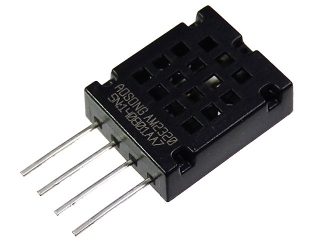
\includegraphics[width=60mm]{images/AM2320.jpg}
        \end{center}
        \caption{温湿度センサモジュール AM2320}
        \label{fig:one}
    \end{minipage}
    \begin{minipage}{0.5\hsize}
        \begin{center}
            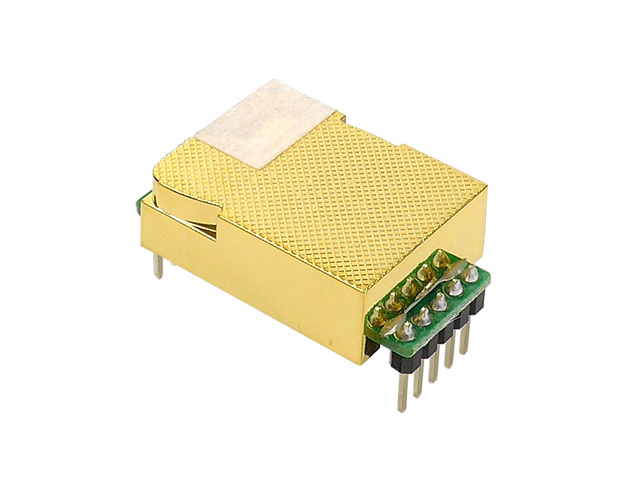
\includegraphics[width=80mm]{images/MH-Z19.jpg}
        \end{center}
        \caption{CO2センサモジュール MH-Z19C}
        \label{fig:two}
    \end{minipage}
    \begin{center}
        ※ 画像は秋月電子通商 商品ページから引用
    \end{center}
\end{figure}
\subsubsection{センサとの接続}
ラズベリーパイと各センサについては以下のように接続されている。
\begin{figure}[htbp]
    \begin{center}
        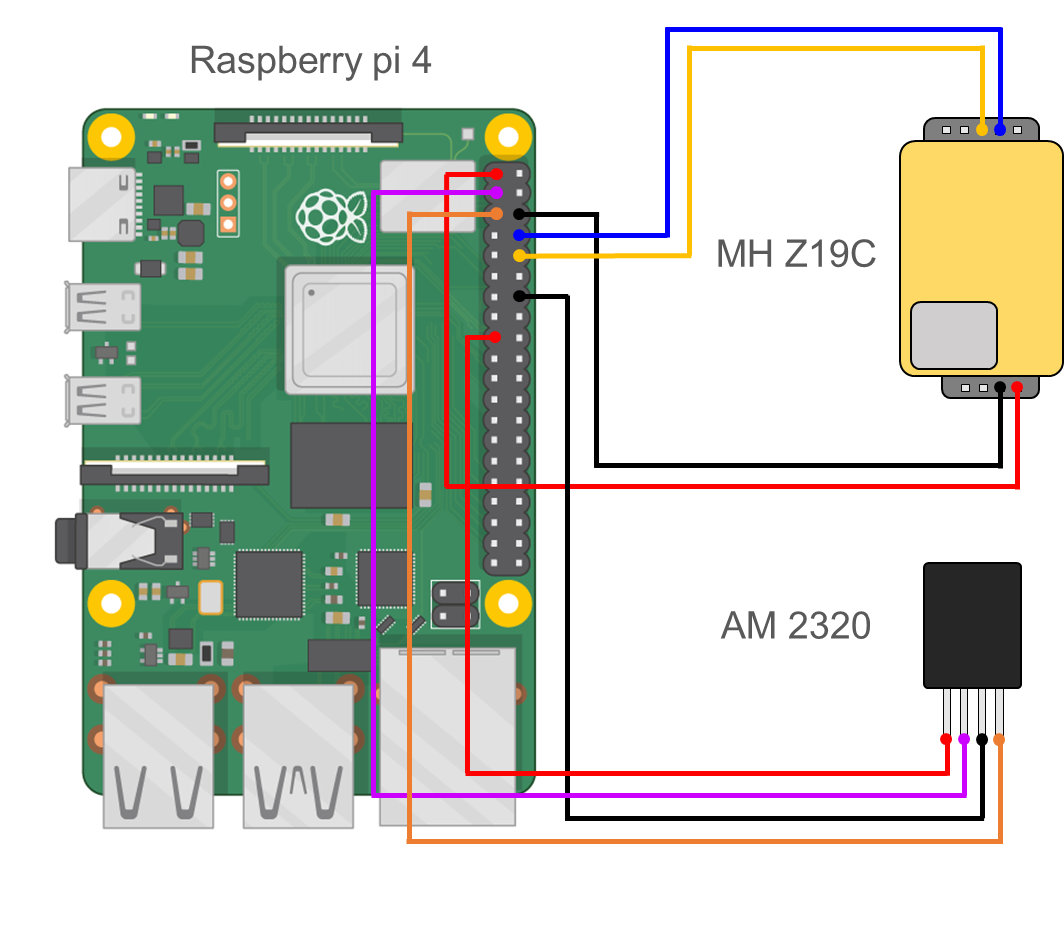
\includegraphics[width=100mm]{images/raspberry-pi_2.png}
        \caption{ラズパイとセンサの接続}
    \end{center}
    \begin{center}
        ※ ラズパイのイラストはラズパイ公式サイトから引用
    \end{center}
\end{figure}
\subsection{表示方法}
表示方法に含む機能として、情報を素早く・的確に伝達できることが挙げられる。
そこで、ラズパイをサーバとして使用し、インターネットを介して、
PC・タブレット・スマートフォンから確認できるようにした。
これにより、デバイスを問わず確認することができ、
複数の接続・表示にも対応しており、場所を問わず確認することができるため、
目的の機能であった情報の伝達機能は達成されると考える。\\
また、飲食店・商業施設で利用する場合は、URLのQRコードを施設内に設置しておけば
利用者がより簡易にアクセスできるため、より情報伝達効果が高まると考えられる。
\begin{figure}[htbp]
    \begin{minipage}{0.6\hsize}
        \begin{center}
            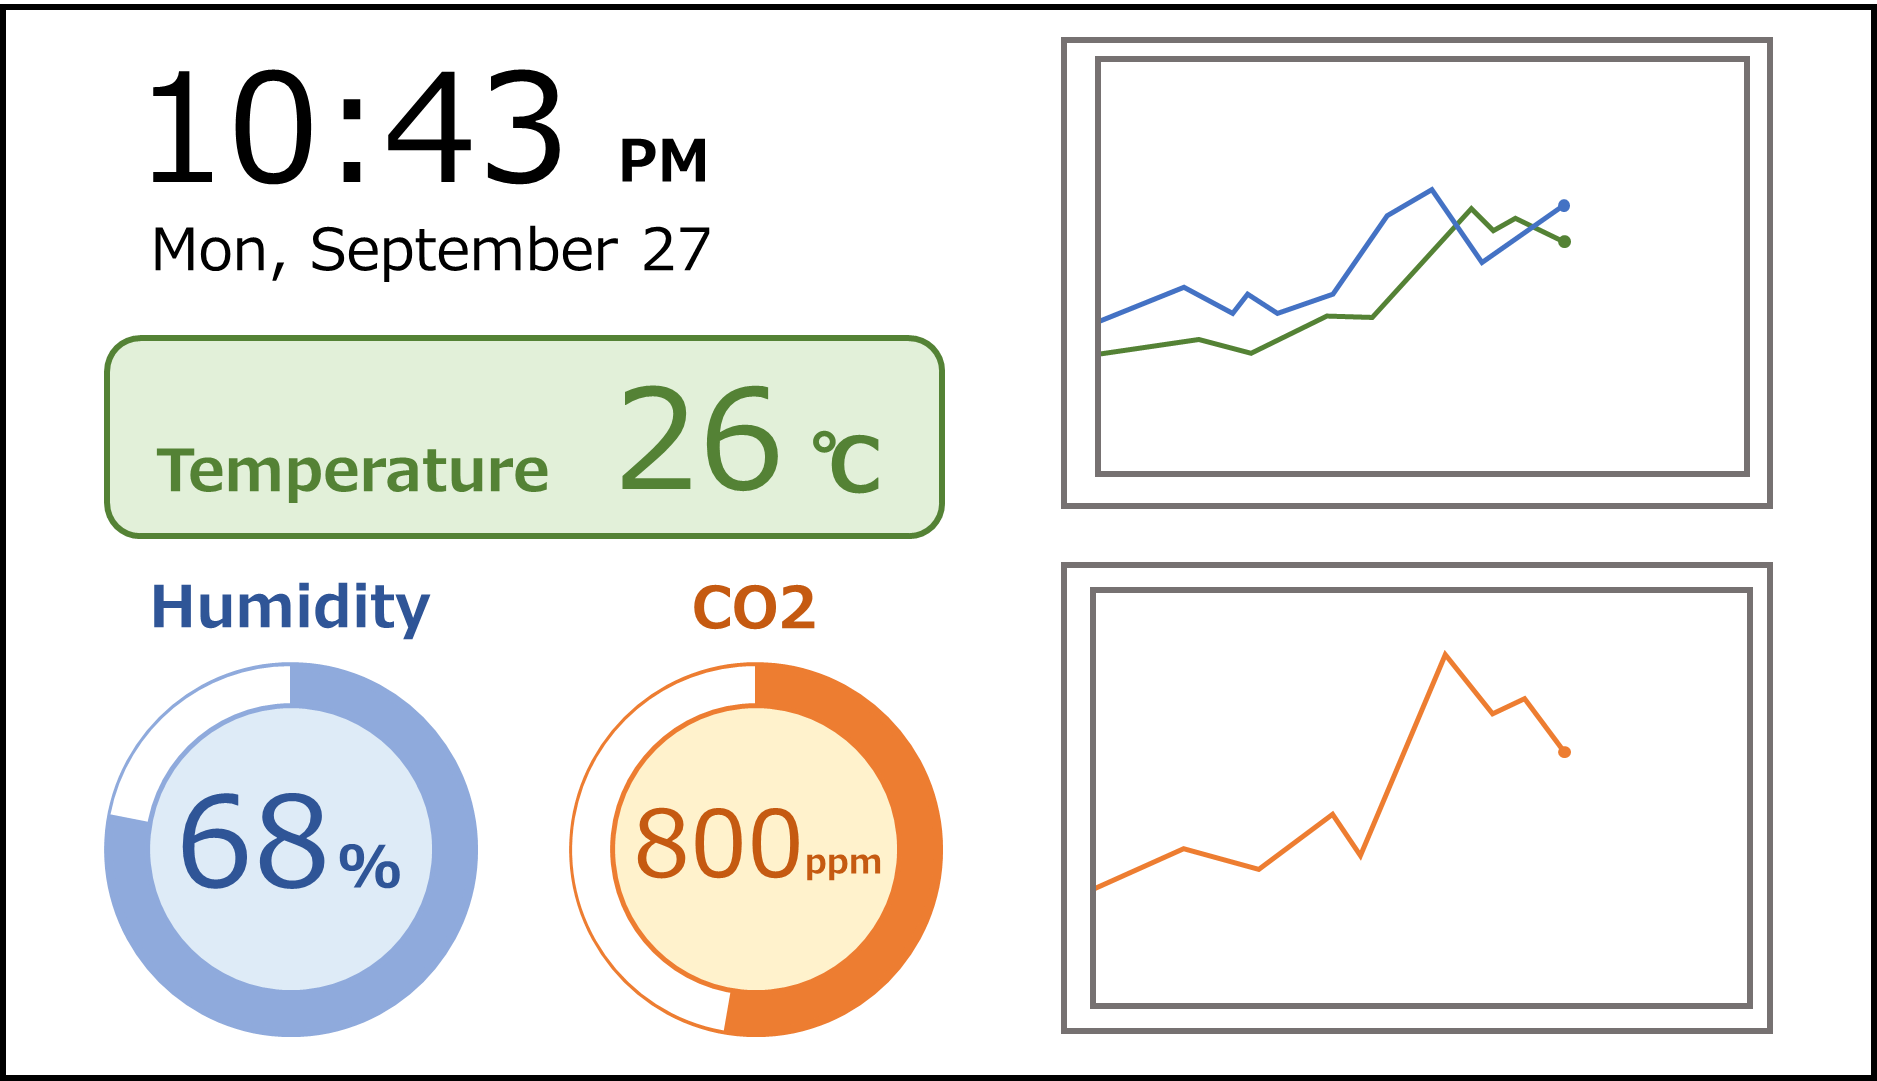
\includegraphics[width=90mm]{images/sketch1.png}
        \end{center}
        \caption{表示画面のスケッチ(PC・タブレット用)}
        \label{fig:one}
    \end{minipage}
    \begin{minipage}{0.4\hsize}
        \begin{center}
            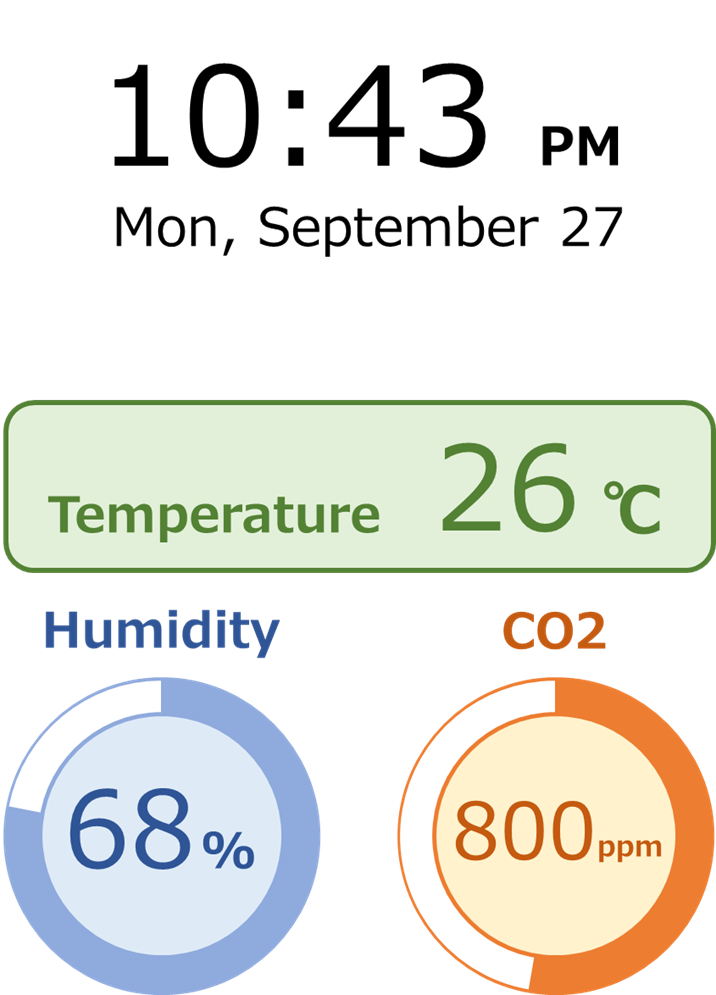
\includegraphics[width=40mm]{images/sketch2.png}
        \end{center}
        \caption{表示画面のスケッチ(スマートフォン用)}
        \label{fig:two}
    \end{minipage}
\end{figure}

\subsection{プログラム}
今回の作品に使用したプログラムについて、以下に示す。
\begin{enumerate}[(1)]
    \item \textgt{センサ値の記録 (毎分)}\\
    1分ごとに、CO2センサ及び温湿度センサからの出力をcsvファイル形式で書き出す。\\
    \item \textgt{時間平均値の計算 (毎時59分)}\\
    毎時59分に、該当する時間(0~59分)のCO2量・温度・湿度の各項目の平均値を算出しcsvファイル形式で書き出す。\\
    \item \textgt{グラフの作成 (毎時59分)}\\
    毎時59分に、時間平均を出力したcsvファイルを読み込み、グラフを作成し、画像ファイルとして書き出す。\\
    \item \textgt{HTML・CSSの作成 (毎分)}\\
    1分ごとに、csvファイルとして出力された各センサの値・時間平均値の推移を示したグラフの画像ファイルを使用してHTML・CSSを書き出す。
    HTMLファイルに自動更新する設定を書き込むことで、新たに生成されたHTMLファイルを読み込み、センサ値が更新される。
    また、CSSについては各センサ値を囲う円グラフの割合を計算し、出力している。\\
\end{enumerate}
\begin{figure}[htbp]
    \begin{center}
        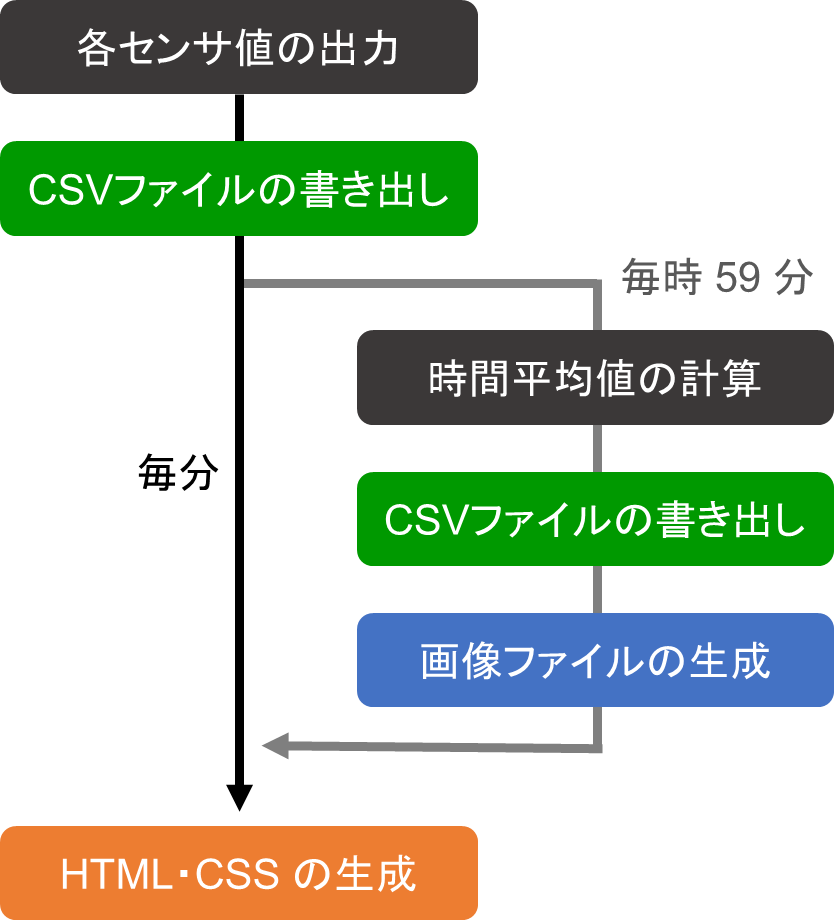
\includegraphics[width=100mm]{images/programs.png}
        \caption{プログラムの動作順番}
    \end{center}
\end{figure}
\subsection{Webサーバ}
ラズベリーパイをwebサーバとして利用する際には、一般的に Apache もしくは Nginx が利用されるようだ。
どちらもオープンソースソフトで展開されており、無料で利用できる。\par
ここで、不特定多数の利用者が考えられる今回の作品では、
高速で負荷に強く、同時接続できるデバイス数も大きいということから、Nginx を採用した。
\section{試用結果}
\begin{figure}[htbp]
    \begin{center}
        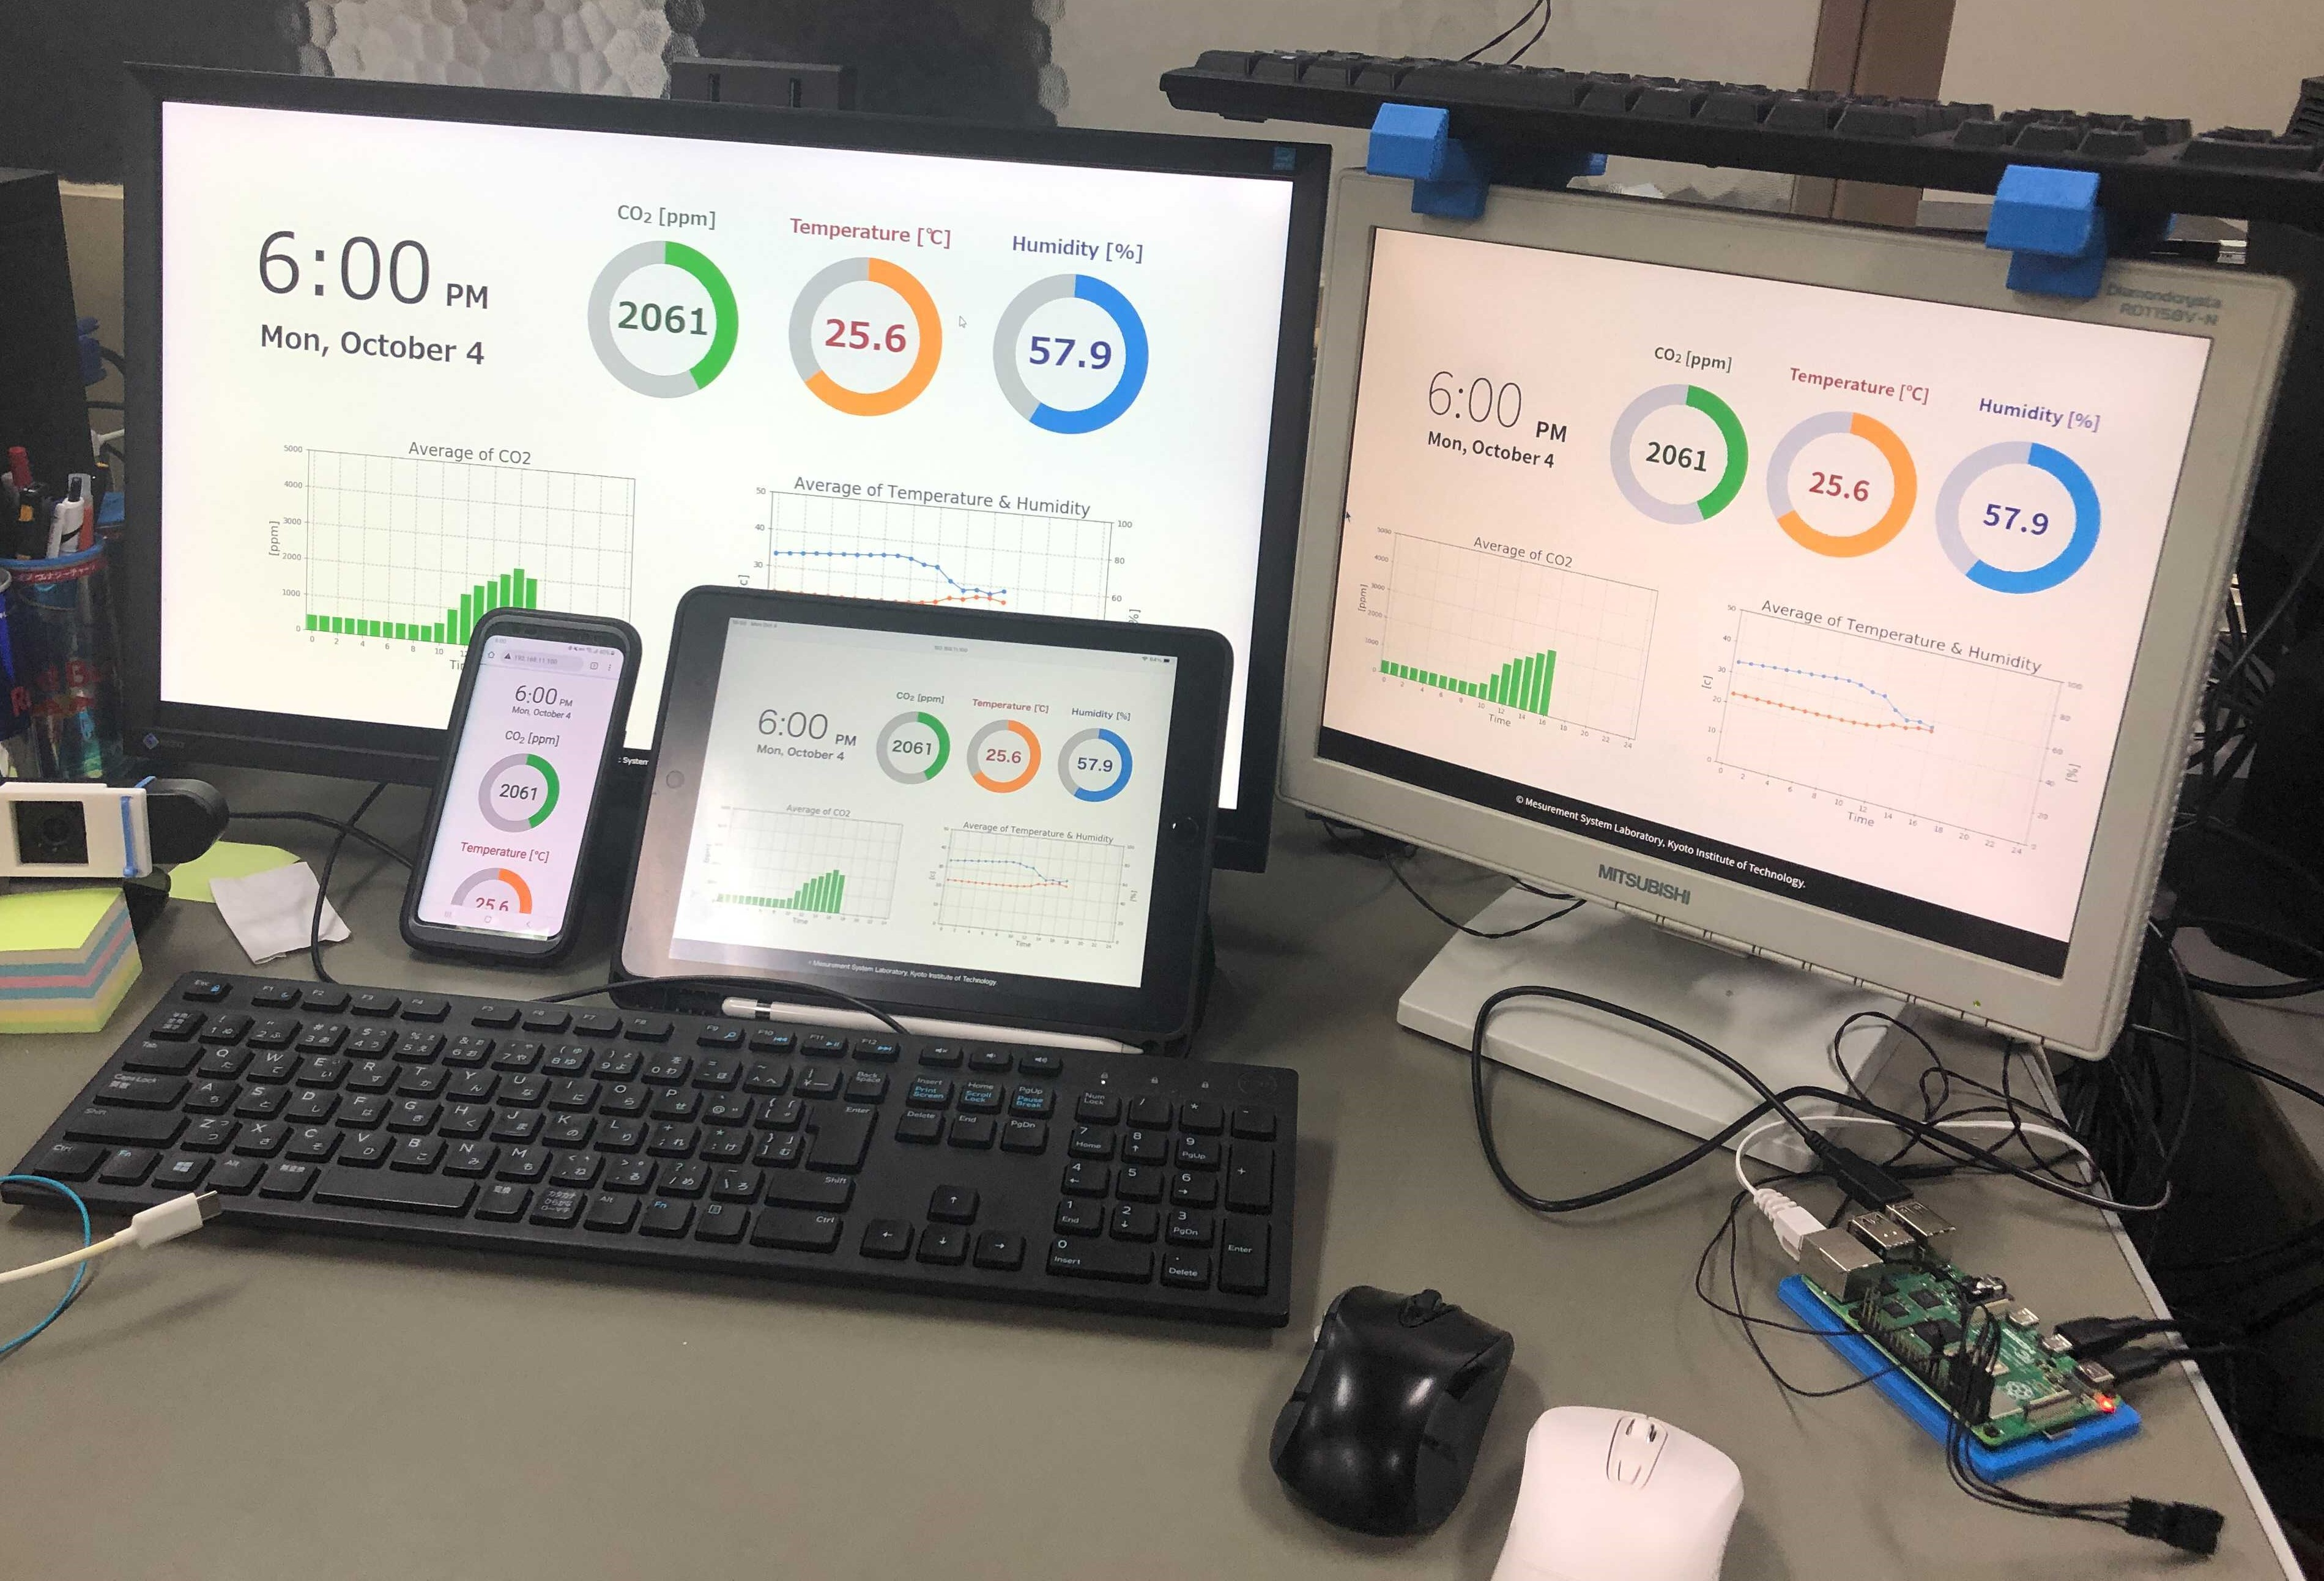
\includegraphics[width=140mm]{images/image.jpg}
        \caption{完成したラズパイサーバと各デバイスの表示}
    \end{center}
    \begin{center}
        ※ 左から順位に、大型ディスプレイ(16:9)、スマートフォン、タブレット、中型ディスプレイ(4:3)
    \end{center}
\end{figure}
実際に2021年10月3日(日)~10月5日(火)に試運転を行ったところ、システムは不具合なく動作したことを確認した。
また、CO2の推移を見ると10月4日及び10月5日の記録において、午後2時頃には2000[ppm]近くを推移しており、
感染症対策を適切に行っていたと考えていたが、実際は非常に換気状態が悪いことがわかった。
ここで、研究室内の窓を約20cm程度開けておくことで、CO2量が大幅に低下し、1000ppmを下回る結果となり、
換気の有効性が確認できた。\par
\begin{figure}[htbp]
    \begin{center}
        \fbox{
        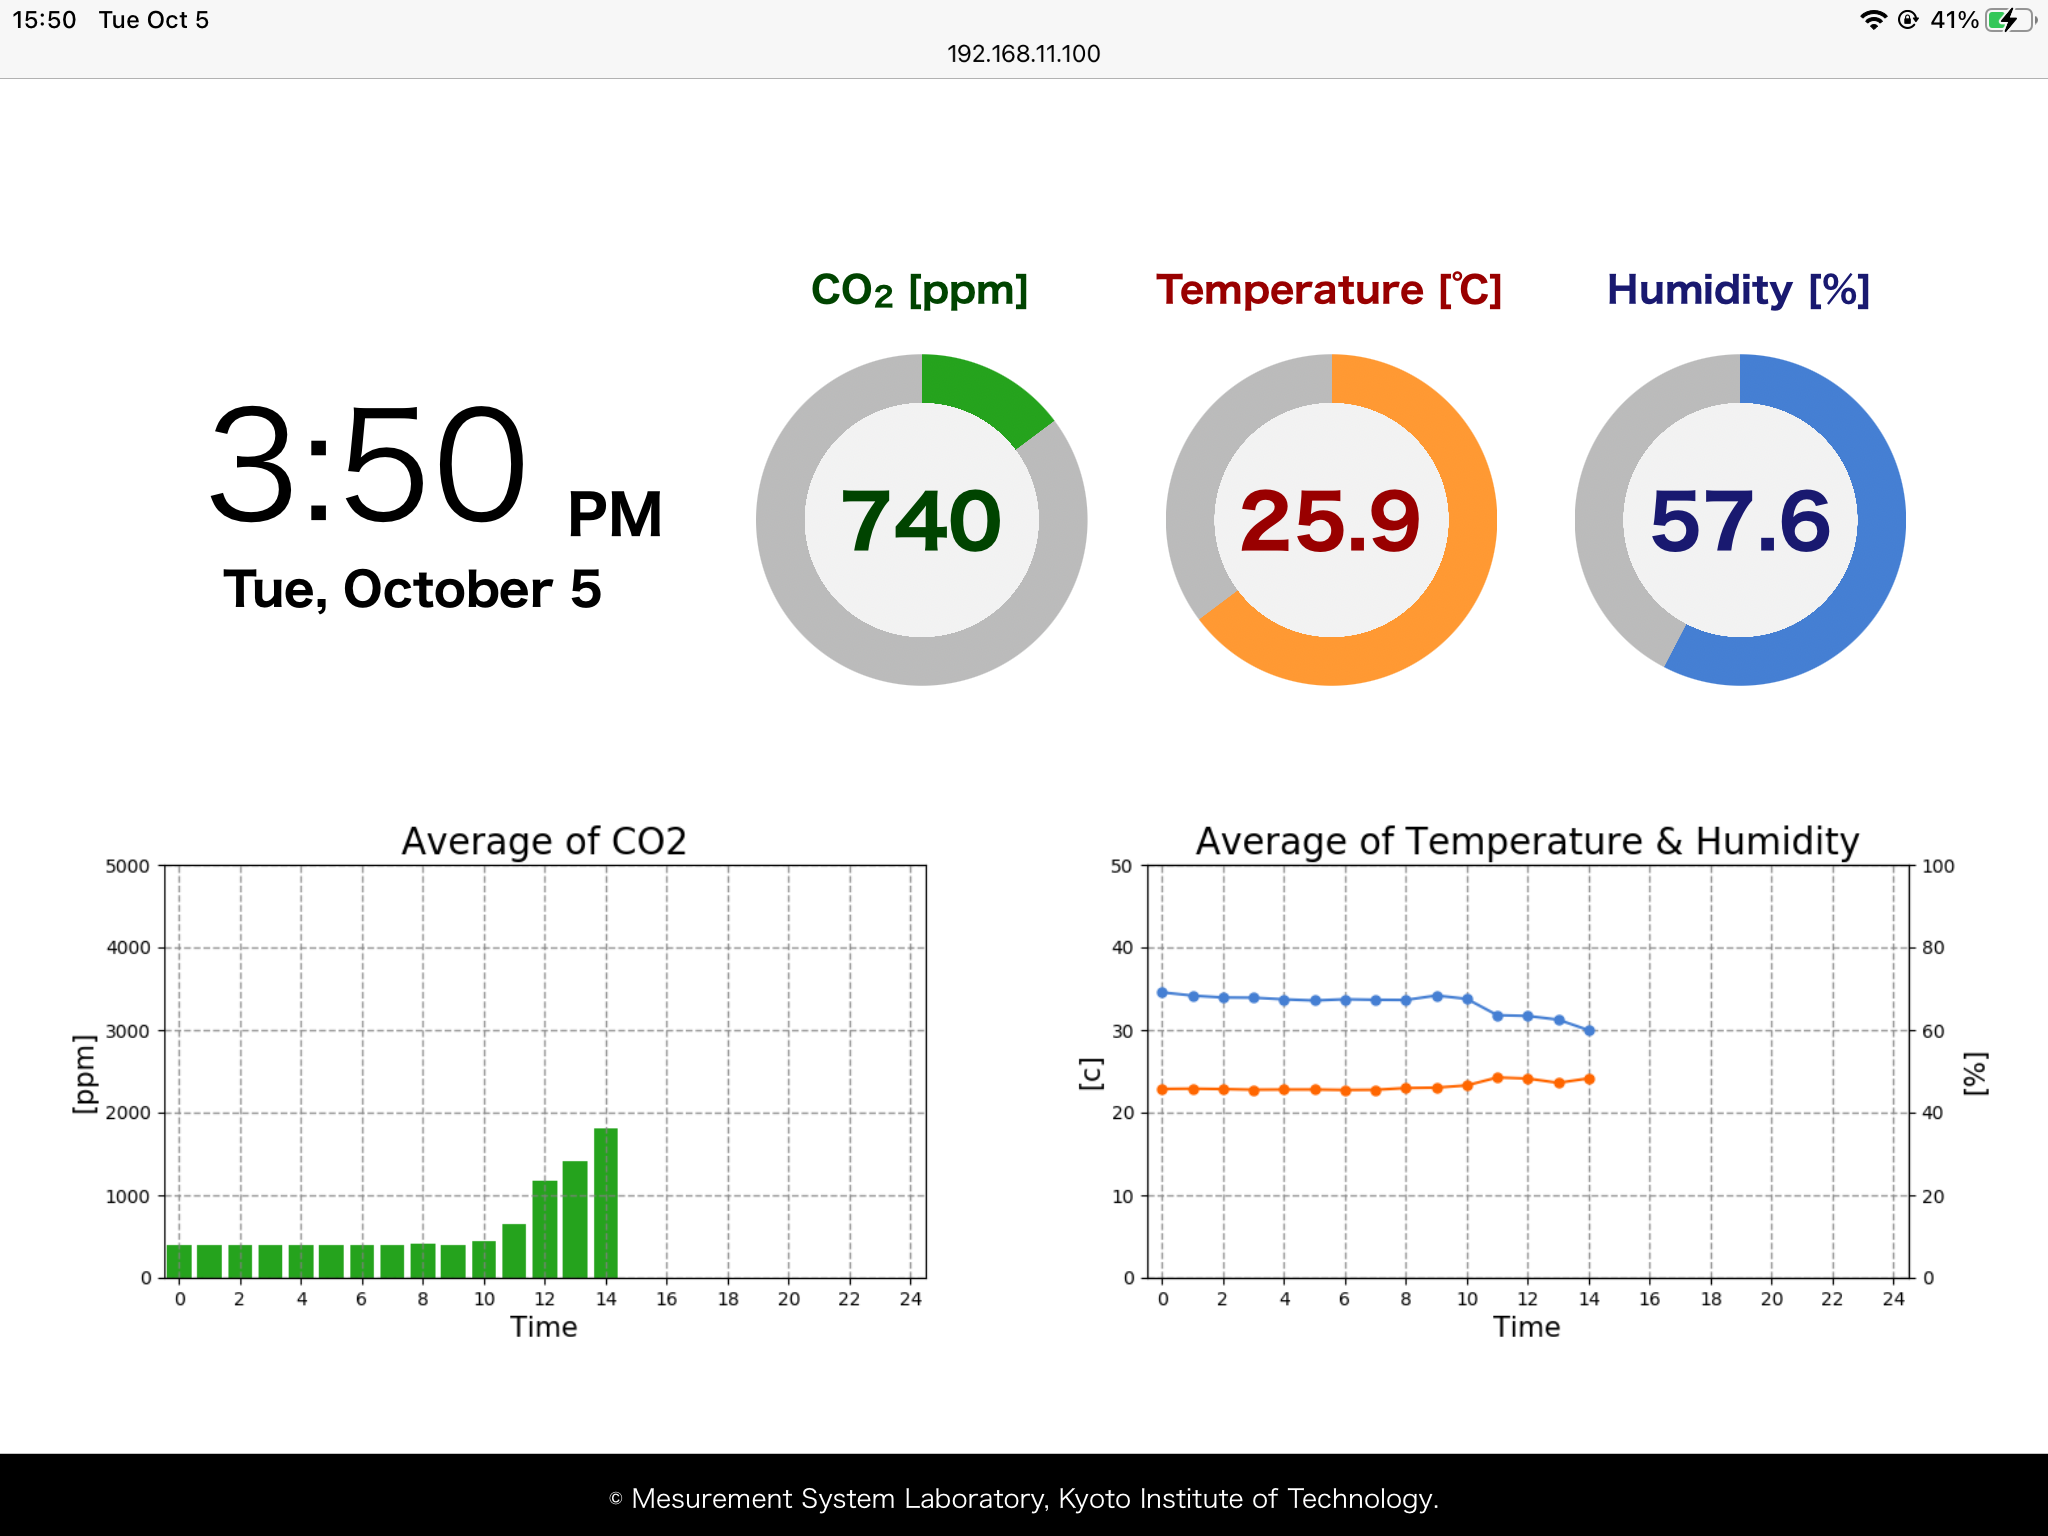
\includegraphics[width=140mm]{images/ipad.png}
        }
        \caption{実際の画面表示(ipad safari)}
    \end{center}
\end{figure}
同様の状況が、他の施設内でも発生している可能性があると考えられ、特に飲食店や商業施設でない、
会社のオフィスや学校の教室等では数値に基づいたガイドラインが設定されていないことも考えられるため、
そのような施設においてもこの作品が有効活用できると考えられる。
\section{今後の展望}
今回の提出では、ラズパイをサーバとしてCO2量及び温湿度を測定し、ブラウザ経由で表示することに成功したが、
今後この作品をより良いものにするために次のようなことを考えている。
\subsection{ケースの作成}
現状では、ラズパイとセンサはむき出しとなっており、落下やものがぶつかった際に破損する恐れがあり、
見た目も不格好であるため、センサとラズパイをコンパクトに収められるケースの作成を考えている。
その際には、温度センサについてはラズパイの廃熱の影響が出ない位置に設置する等、
CO2センサ及び温湿度センサの配置を考慮して設計する必要がある。
\subsection{複数のセンサとの同期}
現在のシステムでは、1つのシステム周辺の観測しかできないため、
大型商業施設等の大きな面積を持つ施設では、効果は小さくなる。
そこで、複数のセンサを配置し、それぞれのデータを取得した後、
データを同期して平均値を算出しそれを用いることで、より一般的な利用が可能となると考える。
\subsection{製作マニュアルの作成・公開}
今回は、飲食店や商業施設での使用を想定した作品としたが、アイディアのみにとどまらず
実際にこの作品を利用してもらえるような方法を考えている。
飲食店・商業施設での利用はもちろん、会社のオフィスや小・中学校の教室等での利用も可能であり、
実際に製作・試用した結果、有効利用できる範囲は大きいと考えられる。
また、夏休みの自由研究といった教育活動の一部としても製作できるような作品にしたい。\par
そのため、今後、電子工作初心者にも簡単に製作してもらえるよう、製作マニュアルの作成に取り組み
研究室のHPを介して公開することを目標としている。
\subsection{製作動画の撮影・公開}
同様に、現在は動画ファイルの公開もYoutube等を介して簡単に行うことができるので、
製作動画及び作品紹介動画を作成し、公開することを目標としている。\\
今回は作品紹介動画を以下のURLのGoogle Driveにアップロードする。\\
URL : \url{https://drive.google.com/drive/folders/1s4Jg9FMNB7ylTQw6h3FbaKY40ksv9tc6?usp=sharing}
\begin{figure}[htbp]
    \begin{center}
        
\includegraphics[width=60mm]{images/QR_drive.png}
        \caption{Google Drive のQRコード}
    \end{center}
\end{figure}
\section{製作に使用したもの}
作品に使用した製品・材料、ソフトウェア、言語を以下に示す。
\subsection{材料・製品}
\begin{center}
    \begin{tabular}{|p{70mm}|p{30mm}|p{30mm}|}
        \hline
        \multicolumn{1}{|c|}{\textgt{材料・製品名}} &\multicolumn{1}{|c|}{\textgt{購入先}}& \multicolumn{1}{|c|}{\textgt{価格(税込) [円]}} \\ \hline
        Raspberry pi 4 Model B 8 GB (element14版)    &                   秋月電子通商                &                        10800                        \\ \hline
        CO2センサモジュール MH-Z19C & 秋月電子通商                                  &                                             2480   \\ \hline
        温湿度センサモジュール AM2320 & 秋月電子通商                                  &     600                                           \\ \hline
        スイッチングACアダプターTYPE-C & 秋月電子通商                                  &                                              900  \\ \hline
        HDMI - VGA 変換アダプタ &      amazon                             &                                                1513\\ \hline
        マイクロHDMI - HDMI 変換アダプタ&     amazon                              &                                             706   \\ \hline
        &                                   & 合計 16099 円                                        \\ \hline
    \end{tabular}\\
\end{center}
\begin{center}
    ※ ディスプレイ・ジャンパワイヤー等は別途購入する必要がある。
\end{center}
\subsection{ソフトウェア}
\begin{center}
    \begin{tabular}{|p{70mm}|p{30mm}|}
        \hline
        \multicolumn{1}{|c|}{\textgt{ソフトウェア名}} & \multicolumn{1}{|c|}{\textgt{用途}} \\ \hline
        Raspbian                                      & OS                                  \\ \hline
        Nginx                                         & Webサーバー                         \\ \hline
    \end{tabular}
\end{center}
\subsection{言語}
\begin{center}
    \begin{tabular}{|p{70mm}|p{30mm}|}
        \hline
        \multicolumn{1}{|c|}{\textgt{言語名}} & \multicolumn{1}{|c|}{\textgt{種類}} \\ \hline
        Python 3                              & プログラミング言語                  \\ \hline
        HTML                                  & マークアップ言語                    \\ \hline
        CSS                                   & マークアップ言語                    \\ \hline
    \end{tabular}
\end{center}
\section{参考資料}
\begin{enumerate}[(1)]
    \item 内閣官房 新型コロナ対策HP : \url{https://corona.go.jp/}
    \item 文部科学省 業種別ガイドライン :\url{https://www.mext.go.jp/a_menu/coronavirus/mext_00028.html}
    \item 一般社団法人 日本フードサービス協会HP : \url{http://www.jfnet.or.jp/contents/safety/} 
\end{enumerate}
\end{document}